\section{Design Goals and Overview}\label{sec:overview}

\begin{figure*}
  \centering
  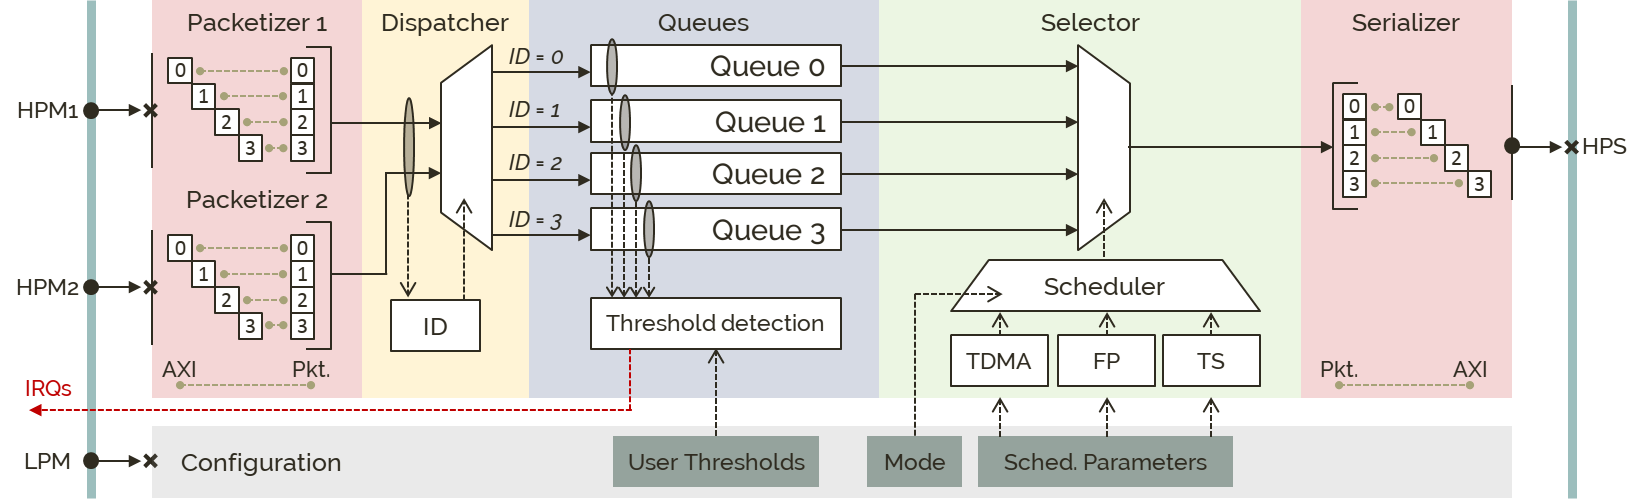
\includegraphics[width=0.8\textwidth]{images/SchIM_diagram.png}
  \caption{Internal logic organization of the \schim connected to the
    PS through the HPM, LPM and HPS ports.}
  \label{fig:MemorEDF_module_schema}
\end{figure*}

%% General introduction about the SchIM
In this section, we introduce the proposed \schim design and describe
the overarching goals of this work. We then provide a bird's-eye view
of the \schim organization and principles of operation.

\subsection{Design Goals}\label{sec:design_goals}
As briefly surveyed in Section~\ref{sec:relwork}, there have been
numerous proposals for better memory controllers and approaches to
manage memory traffic in modern multi-core embedded platforms. With
respect to the existing literature, the purpose of this work is
twofold. First, we want to demonstrate that scheduling CPU-originated
memory traffic at the granularity of individual transactions is
possible in PS-PL platforms. Second, and more importantly, we want to
provide an infrastructure that is generic and extensible enough for
the broader research community to adopt and foster a new chapter on
PL-assisted memory scheduling. With this in mind, we establish the
following goals.

\par{\bf Extensible memory scheduling infrastructure.} First and
foremost, the \schim has been designed with modularity and
extensibility in mind. We separate the functionalities that concern
handling, queuing, selection, and forwarding of memory requests inside
our infrastructure. Moreover, we design our \schim to be able to support multiple memory scheduling policies simultaneously. A simple,
standardized interface is provided to define new memory scheduling
policies without impacting the design of the rest of the \schim. We
discuss in Section~\ref{sec:sched_interf} the generic interface
provided by the \schim to implement a new memory scheduling policy.

\par{\bf Runtime configuration and transparency.} We want the \schim
to be a robust supporting infrastructure to evaluate, compare, and
contrast memory scheduling policies. As such, we strive to provide (1)
runtime reconfigurability and (2) operational transparency. It is possible to rapidly identify desirable configuration parameters by
allowing memory scheduling policies to be switched at runtime. Besides, an adopted policy can be tuned according to the workload criticality and memory intensiveness. For this purpose, the \schim exposes a memory-mapped
configuration interface where all the operational parameters can be
changed at runtime. At the same time, we want to ensure that the
applications and the (real-time) operating system under analysis need
not be modified to use the \schim. Hence, we propose using a
thin virtualization layer to selectively route memory traffic through
the \schim without changes to the binary of OS kernel and
applications.

\par{\bf Realistic performance with experimental policies.} One of the
limiting factors of research on memory scheduling policies is the
ability to construct evidence of performance improvements with
the realistic workload. Proposing a new memory scheduling policy is
traditionally done with either a simulated setup or with a
full-system soft-core implementation. Both cases are considerably slower than what it would be in real systems and force the use of an unrealistically lightweight workload. Nonrealistic workloads limit the repeatability of experiments of scale.

Furthermore, the multi-fold drop in performance excludes the
possibility of adopting experimental memory scheduling policies for a
production-ready system. Conversely, we envision that our \schim will
be an intermediate step in the transition path to the production of
research-seeded ideas. Additionally, as PS-PL platforms mature and the interplay of PL and memory resources improves, a \schim-like design
could be the way to go for mission-reconfigurable, upgradable embedded
systems.

\subsection{Design Overview}
As previously mentioned, the \schim leverages the PLIM
approach. CPU-originated main memory transactions are re-routed
through the programmable logic and scheduled by the \schim according
to a flexible and configurable policy. The result is that the timing
of memory transactions generated by real-time applications can be
carefully determined and reasoned upon. Because the \schim follows a
PLIM approach, transactions can be selectively sent to the \schim for
scheduling. However, it is always possible to dynamically exclude the
\schim and route transactions directly to the main memory. Toward this paper's incentive, we consider a setup in which \schim handles all the CPU-generated memory transactions.

%% First and foremost, SchIM follows a selective and dynamic re-routing
%% policy settled at the runtime, meaning that provided a proper routing
%% configuration interface, SchIM can be bypassed if unacceptable
%% overhead for some applications is detected by going through the PL
%% following the Loop-Back routing strategy. Additionally, SchIM,
%% provides a safe production-ready environment on COTS platforms where
%% one can enfroce and test any proposed scheduling policy at the level
%% of the transaction altogether by the real hardware. Memory scheduling
%% traditionally done via hardware modifications at the controller level,
%% or solely via software. Providing SchIM, we are now able to transcend
%% this on intact COTS to conduct an analysis of feasibility, challenges
%% and performance.

\fig{fig:PS-PL-diagram} provides an overview of the location of the
\schim in the reference platform, while its internal organization is
visible in \fig{fig:MemorEDF_module_schema}. Application memory
requests reach the \schim the aforementioned HPM ports. Without loss
of generality, we consider a \schim instance with two arrival lanes,
which are labeled as \axiin{1} and \axiin{2} in
\fig{fig:MemorEDF_module_schema}. The \schim then forwards the
received transactions towards main memory through the \axiout{}
interface. A more detailed view of the \schim module is provided in
\fig{fig:MemorEDF_module_schema} where the same convention is used to
identify input and output ports. In addition, as shown in
\fig{fig:MemorEDF_module_schema}, a fourth \axiconf{} port is used to
configure the \schim from the PS.

%% The objective of the module is to arbitrate the access of the bus to
%% the main memory between the different cores of the PS side at the
%% transaction level by enforcing a given policy.  Roughly, the module
%% receives transactions from the PS side, acknowledges them and finally
%% repeat them with the main memory as destination.  The exact order in
%% which inter-core transactions are being repeated is decided by an
%% embedded on-chip hardware scheduler.

%% \begin{figure}
%%   \centering
%%   \begin{tikzpicture}[scale=0.6, every node/.style={scale=0.6}]
    % Modules
    \draw[fill={rgb:black,1;white,7}] ( 0.0, 0.0) rectangle ( 4.0, 4.0) node[pos=.5] {PS};
    \draw[fill={rgb:black,1;white,7}] ( 6.0, 0.5) rectangle ( 8.0, 2.5) node[pos=.5] {SchIM};
    \draw[fill={rgb:black,1;white,7}] (10.0, 0.5) rectangle (12.0, 2.5) node[pos=.5] {Bleacher};
    % Outline PL
    \draw[dashed] ( 0.0, 4.0) -- ( 4.0, 4.0) -- ( 4.0, 0.0) -- (14.0, 0.0) -- (14.0, 6.0) -- ( 0.0, 6.0) -- ( 0.0, 4.0);
    % Buses
    % PS to SchIM HPM0
    \draw[{Stealth}-{Stealth}] ( 4.0, 1.5) -- ( 6.0, 1.5) node[above, pos=.5] {Transactions};
    % SchIM to Bleacher HPM0
    \draw[{Stealth}-{Stealth}] ( 8.0, 1.5) -- (10.0, 1.5) node[above, pos=.5] {Transactions};
    % SchIM to Bleacher HPM0
    \draw[{Stealth}-{Stealth}] (12.0, 1.5) -- (13.0, 1.5) -- (13.0, 5.0) -- ( 2.0, 5.0) node[above, pos=.5] {Transactions} -- ( 2.0, 4.0);
    % PS to SchIM and Bleacher LPD
    \draw[{Stealth}-{Stealth}] ( 4.0, 3.0) -- (11.0, 3.0) node[above, pos=.5] {Configuration} -- (11.0, 2.5);
    \draw[-{Stealth}] ( 7.0, 3.0) -- ( 7.0, 2.5);
\end{tikzpicture}

%%   \caption{High-level block design of the proposed \schim
%%     module. \emph{RM: we need to replace this picture with one that
%%       provides more details about the main blocks of the platforms. We
%%       also do not need to include the bleacher as it is not
%%       fundamental for the operation of the \schim.}}
%%   \label{fig:SchIM_overview_schema}
%% \end{figure}


%% Micro-architecture and first list of modules
The \schim module is composed of a number of sub-modules grouped into
three different domains, namely (i) the \emph{interfacing domain},
(ii) the \emph{queuing domain}, and (iii) the \emph{scheduling
  domain}.

\par{\bf The interfacing domain} encompasses the sub-modules to
interface the core logic of the \schim with the rest of the system
using the AXI protocol.  This is comprised of three sub-modules. These
are (i) the \emph{packetizer(s)}, (ii) the \emph{serializer}, and
(iii) the previously mentioned \emph{configuration} interface.

The PS-facing end of the {\bf packetizer} offers an AXI slave port to
accept new incoming transactions. Upon receipt, this module transforms
each transaction into an equivalent \emph{packet} that can be queued
and scheduled by \schim. Packetization of AXI
transactions is necessary to be able to store transactions that are
serial by nature.  A standard AXI transaction is composed of
one address phase (AR or AW channel) followed by a data phase (R or W
channel), which can be itself composed of multiple successive bursts.

In many ways, the {\bf serializer} is the dual module of the
packetizer. Its purpose is to transform the packets that encode
CPU-generated memory requests back into AXI-compliant transactions. As
such, the serializer offers a master port to the rest of the system to
be routed to the main memory controller.

%% purpose of slave and master ports, they are also in charge of
%% respectively transforming the AXI transactions into an equivalent
%% packet and to transform these packets 

\par{\bf The queuing domain} handles how packets are stored between
receipt and re-trasnmission. This domain is comprised of (i) the
\emph{dispatcher} module, (ii) the \emph{transaction queues}, and
(iii) the \emph{selector} module.

The use of {\bf multiple transaction queues} is necessary to
differentiate the traffic of the CPUs and perform scheduling. As such,
the \schim associates a queue to each of the active cores --- four in
the platform of reference.
%% Therefore, in order to cancel the Round Robin arbitration policy
%% applied in the PS side and in order to avoid that one high priority
%% core is stalled by a lower priority one, each core is granted a queue
%% within the \schim module. <-- This should be obvious (RM)
The queues implemented in the \schim not only act as a holding space
for in-flight memory transactions.  They also (a) provide information
to the scheduling domain regarding their current state, and (b) they
can generate a congestion control signal to the associated CPU
core.

Congestion control is vital because memory transactions originated
at the LLC controller follow the same route to the \schim regardless
of the originating CPU. Typically, the total number of outstanding
transactions that the cores can emit exceeds the queuing elements' capacity on the loop-back route. Hence, priority inversion arises if a low-priority CPU's memory traffic is (temporarily) held. Latter is due to the uncontrolled queue buildup, which provokes a head-of-line blockage. Importantly, what described is true also for the normal
route and it is a direct consequence of the best-effort nature of
traditional multi-core memory buses. The \schim allows the user to
specify a configurable threshold on the occupancy of the queues that,
when reached, issues a regulation signal to the corresponding CPU. We
describe in greater detail how congestion control was implemented on
the target platform in Section~\ref{sec:pl-to-ps-feedback}.

As suggested by \fig{fig:MemorEDF_module_schema}, transactions are
categorized and enqueued based on the source of traffic. The {\bf
  dispatcher} module performs the matching between an incoming
transaction and the destination queue. Similarly, transactions are
dequeued by the {\bf selector} module and sent directly to the output
of the \schim following the scheduling domain's resolutions.

\par{\bf The scheduling domain} encompasses all the sub-modules that
enable arbitration of transactions issued by the different cores of
the PS. The modules in this domain are intended to be generic for
extensibility, albeit the first set of three template schedulers is
provided as a proof of concept.  The scheduling policies currently
implemented in the \schim are Fixed Priority (FP), Time Division
Multiple Access (TDMA), and Budget-based Traffic Shaping (TS).  Each
of the parameters required by the implemented policies --- such as the
priorities, the periods, and the budgets --- can be adjusted at
runtime via the configuration interface.

The FP scheduler allows associating a priority value to each of the
transaction queues. Pending transactions at the queues are then
forwarded out of the \schim following the user-defined priority
order. The TDMA scheduler allows associating a transmission time slot
to each of the queues expressed in PL clock cycles. The module then
builds a schedule by concatenating the per-core slots so that only
pending transactions from one queue at a time are forwarded by the
\schim. Finally, with the TS scheduler, it is possible to associate a
maximum rate at which transactions from each queue are forwarded by
the \schim. 

%% Finally, the scheduling domain is also the one in charge of the
%% control of the remaining \schim module, driving and selecting the
%% adequate signals and ensuring the coherence and integrity of the data.

%% \subsection{Modules Overview}

%% \par{\bf Packetizer:} The packetizer module transforms transactions on
%% the asynchronous AXI bus into schedulable entities to be queued at any
%% of the \schim queues.

